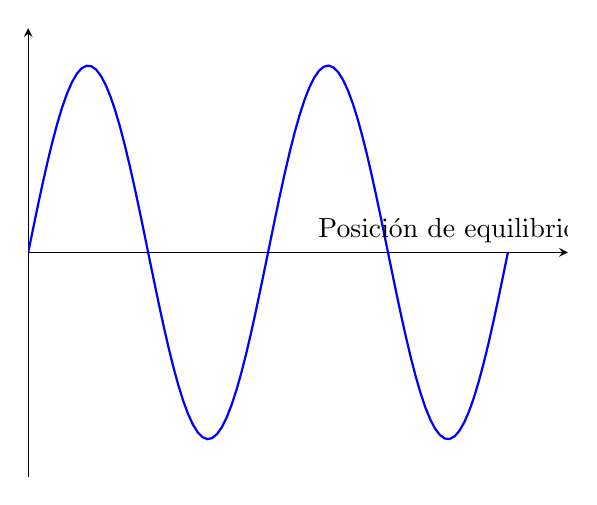
\begin{tikzpicture}
  \begin{axis}[
    xmin=0,xmax=4.5*pi,
    ymin=-1.2,ymax=1.2,
    axis lines=middle,
    xtick={0},
    ytick={0}
    ]

    % Funcion senoidal
    \addplot[color=blue,samples=100,domain=0:4*pi,thick]{sin(deg(x))};

    % Posicion de equilibrio
    \node[above] at (axis cs:7*pi/2,0) {Posición de equilibrio};
  \end{axis}
\end{tikzpicture}
